\chapter{Analysis Optimization}\label{sec:analysis_optimization}
After carefully designing physical objects to represent the final state of a physical process of interest the main task is to construct a quantity that tests the compatibility of the prediction with the observation. Typically this is a kinematic variable such as the invariant mass of the Higgs pair system $m_\text{HH}$ in this analysis, designed to differentiate signal from background. Since the statistical test is based on frequentist statistics as further explained in chapter \ref{sec:statistics} a histogram is constructed from the final quantity. Usually at each step leading to this quantity it is optimized on some ratio of signal to background.

Since the purpose of this quantity is to optimally separate signal from background it is actually better suited to be treated with a \ac{ml} model as already applied widely in particles physics \citep{albertsson2019machine,shlomi2020graph,feickert2021living,Schwartz2021Modern}. These models are typically trained to categorize input events into signal and background(s). However a key issue with signal to background optimization is that they are not optimized for the actual final quantity of interest like a discovery significance or the level of confidence if a tested hypothesis should be accepted or rejected.

While the signal-to-background ratio or the separation ability of the \ac{ml} model may correlate to some extent with the expressivity of the statistical test, it is not optimal, particularly because it does not account for uncertainties that can significantly impact the outcome of the statistical test. This means that even if the statistical test performs exceptionally well on nominal values, its effectiveness may dramatically diminish when presented with inputs that deviate from these nominal values due to uncertainties.

This issue can be addressed with: \textit{\ac{neos}} \citep{Simpson_2023}. It is based on the observation that the classifier training can be done with respect to the actual final quantity of interest by integrating the statistical model into the training.


\section{Machine Learning}
\ac{ml} refers to algorithms that enable computers to learn from data to make predictions for some specific task without being explicitly programmed for \citep{kubat2021introduction}. One particular subset of \ac{ml} are \acp{ann} inspired by the human brain. Their fundamental unit are nodes, the neurons, that are interconnected to several other neurons organized in consecutive layers with an initial input and a desired output as shown in figure \ref{fig:ann}. The signals between neurons are transferred weighted and each neuron has an activation function that converts the received input stimulus into an output strength. Thus learning occurs through adjusting the weights between the neurons. \acp{ann} can be designed in various ways with many layers depending on the specific task.
\begin{figure}
    \centering
    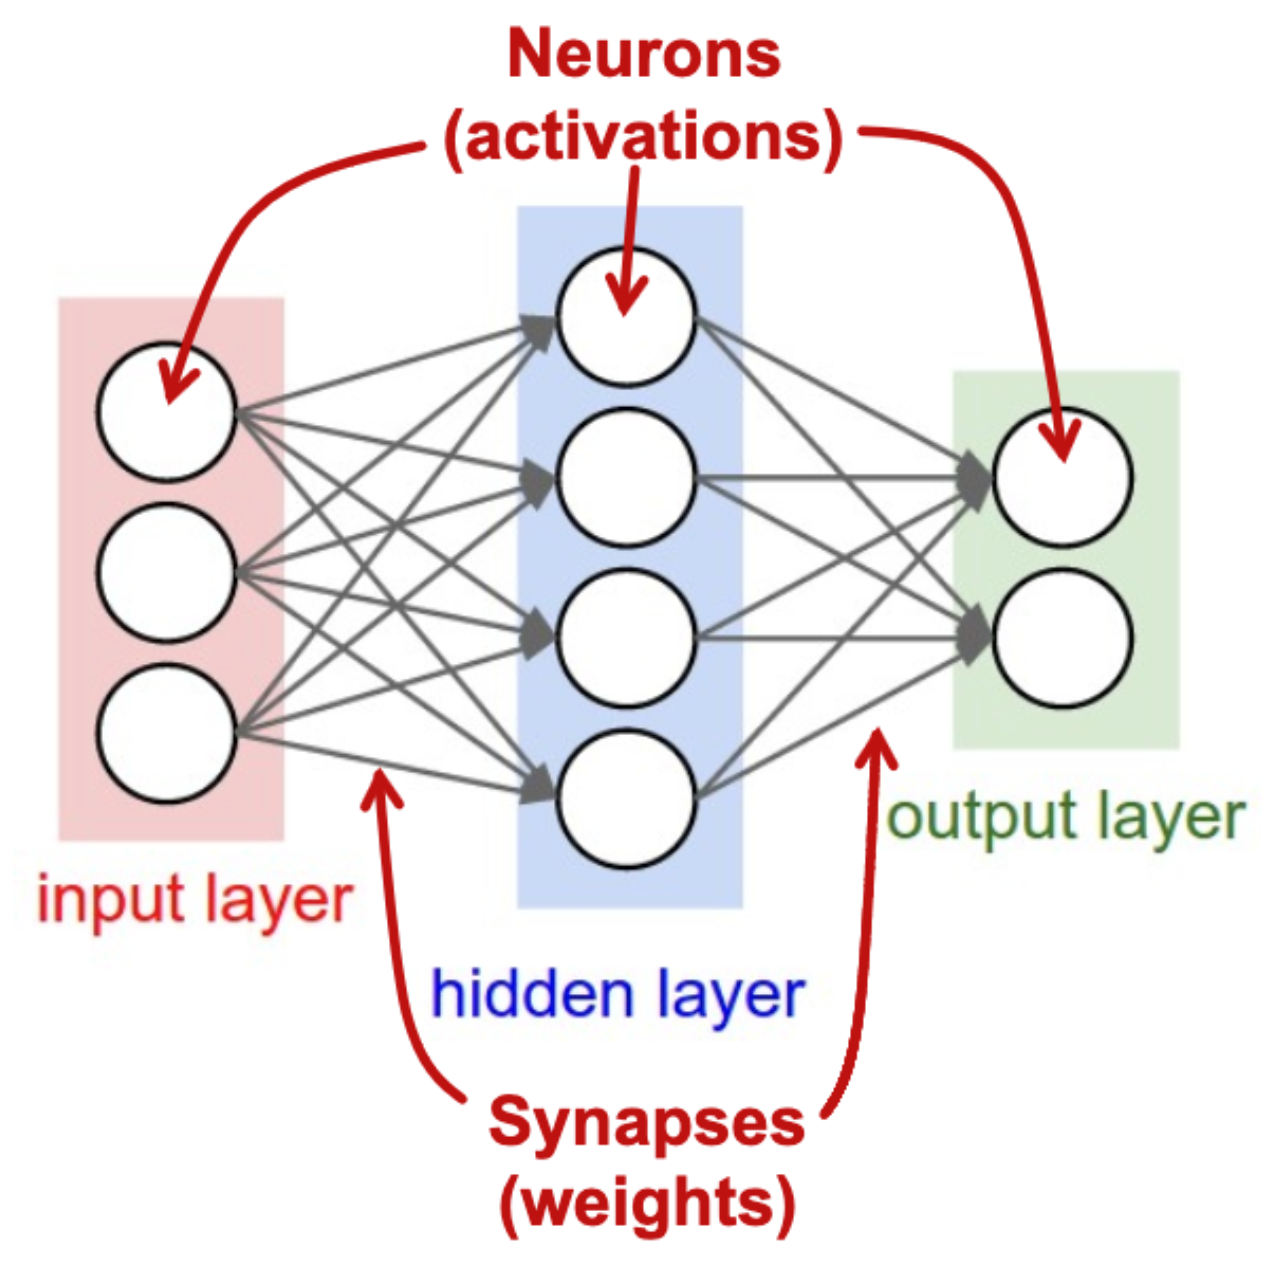
\includegraphics[width=0.4\textwidth]{ann}
    \caption[]{Structure of artificial feed-forward neural networks. Adopted from \citep{8114708}.}
    \label{fig:ann}
\end{figure}

The training of \acp{nn} is usually done with the back-propagation algorithm which seeks to minimize a cost function $C(\bm{\varphi})$ that is designed to measure the deviance of a presented input to a desired output dependent on the model parameters $\bm{\varphi}$. For a feed-forward \ac{nn} these model parameters are the mentioned weights and added biases of the neurons. Via gradient descent the minimum of the cost function can be found stepwise with the first derivative and a chosen learning rate parameter $\gamma$
\begin{equation}
    \bm{\varphi}_{n+1} = \bm{\varphi}_n-\gamma\nabla C(\bm{\varphi}_n).
    \label{eq:grad_descent}
\end{equation}
In three dimensions this corresponds to a mountaineer searching for the valley by going in the direction of the steepest descent with a stepsize proportional to $\gamma$.



\section{NEOS}
The key idea of \acl{neos} is to choose the cost function as the quantity which is to be minimized. In this case the $\mathrm{CL}_s$ value is a reasonable choice as discussed in chapter \ref{sec:statistics}. For a typical analysis chain as shown in figure \ref{fig:neos} this translates into a mathematical concatenation of the individual steps within the chain.
\begin{figure}
    \centering
    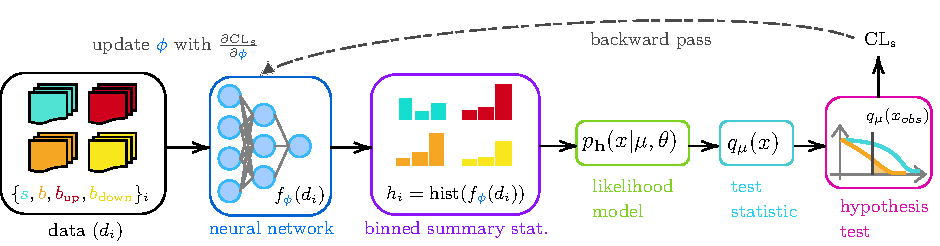
\includegraphics[width=1\textwidth]{neos}
    \caption[]{Typical particle physics analysis chain. For \ac{neos} the $\text{CL}_s$ value is back-propagated to train the neural network parameters $\bm{\varphi}$. Adopted from \citep{Simpson_2023}.}
    \label{fig:neos}
\end{figure}
Hence the cost function $\text{CL}_s$ is a function of the dataset $\mathcal{D}$ and the \ac{ml} model parameters $\bm{\varphi}$
\begin{equation}
    \mathrm{CL}_s = f(\mathcal{D},\bm{\varphi}) = (f_{\mathrm{sensitivity}} \circ f_{\mathrm{test\,stat}} \circ f_{\mathrm{likelihood}}  \circ f_{\mathrm{histogram}}  \circ f_{\mathrm{observable}})(\mathcal{D},\bm{\varphi}).
\end{equation}
In order to find the minimum via the gradient descent of equation \ref{eq:grad_descent} \cls needs to be differentiable with respect to $\bm{\varphi}$. By applying the chain rule this reads for one model parameter $\varphi_i$
\begin{equation}
    \frac{\partial\,\mathrm{CL}_s}{\partial \varphi_i} = \frac{\partial f_{\mathrm{sensitivity}}}{\partial f_{\mathrm{test\,stat}}}\frac{\partial f_{\mathrm{test\,stat}}}{\partial f_{ \mathrm{likelihood}}} \frac{\partial f_{\mathrm{likelihood}}}{\partial f_{\mathrm{histogram}}}   \frac{\partial f_{\mathrm{histogram}}}{\partial f_{\mathrm{observable}}}  \frac{\partial f_{\mathrm{observable}}}{\partial \varphi_i}.
\end{equation}
Apart from histogramming which is inherently discrete all other steps are differentiable. A method to render histograms differentiable is \ac{kde} \citep{CRANMER2001198}. Instead of counting a quantity in bins, a histogram can be approximated by representing each data point by a normal distribution termed the kernel. This distribution has the mean equal to the the data point's value and a chosen value for the standard deviation, also called the bandwidth in this context. Since the area under each Gaussian is equal to one, the collective addition of all Gaussian's yields a smoothed estimate of a histogram that is inherently differentiable. However, it is crucial to select the bandwidth appropriately, ideally around the desired bin width, as the quality of the KDE estimate is highly sensitive to this choice. This is demonstrated in Figure \ref{fig:relaxed_hist}. Although this can be a source of uncertainty any differentiable step or block in figure \ref{fig:neos} can always be reverted back to the exact calculation.
\begin{figure}
    \centering
    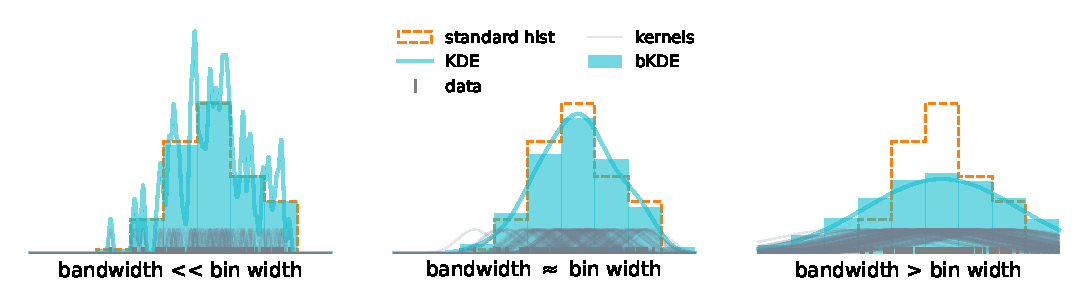
\includegraphics[width=1\textwidth]{relaxed_hist}
    \caption[]{Dependence of the histogram approximation with normal distributions of different standard deviations called bandwidth in the context of \ac{kde}. Depicted in grey small bars on the x-axis are the data points and in grey above them their kernel estimates. Further shown is the standard histogram binned from data, the \ac{kde} and the \ac{bkde} as a histogram calculated from the area under the \ac{kde} in a chosen bin range. Adopted from \citep{Simpson_2023}.}
    \label{fig:relaxed_hist}
\end{figure}


\subsection{Implementation}
Tracing differentiation through software is achievable by recognizing that any software essentially comprises a series of elementary arithmetic operations. Since the analytic solutions for these operations are known, the task reduces to concatenating all these operations and differentiating the resulting function. This is also known as \textit{Automatic Differentiation} and is achieved here with the help of the software package \textsc{jax} \citep{jax2018github}.

While the concept may appear straightforward, one of the challenges that previously hindered its implementation is the difficulty of differentiating across multiple individual software frameworks.That this became feasible within a reasonable time frame builds greatly on the transition efforts  of the individual steps to the \textsc{Python} programming language, moving away from C++ \textsc{ROOT}-based software \citep{ANTCHEVA20092499}. While \textsc{root} was indispensable at its time of emergence it is now less optimal for contemporary scientific analysis. This is because it is not only more difficult to integrate within other current software but also due to its user-unfriendliness compared to \textsc{Python} solutions which are maintained by a broad scientific community doing data-analysis. Using \textsc{python} in this context presents a notable advantage since it benefits from widespread community support and pre-existing solutions to many common problems, enabling the use of tools like \textsc{jax}, which were not originally connected to \ac{hep}.


The original proposers \citet{Simpson_2023} of \ac{neos} developed differentiable versions of common \ac{hep} tasks like the upper mentioned hypothesis test, histogramming and the optimization of a cut in a packaged called \textsc{relaxed} \citep{Simpson_relaxed_version_0_3_0_2023}. They successfully tested the entire pipeline in a toy model \citep{Simpson_neos_version_0_2_0_2021}. These efforts were transferred and further developed to be applicable to this analysis with \citep{hh_neos}.


\red{ this somewhere here, or outlook?
    stack several neural networks together!!! end to end training
    one for pairing, event selection
    stack arbitrarily
    selling point ist binning ist optimiert, auch mit fixen bins
}